%!TEX root = paper.tex

\textbf{Note: There are more h's than v's: $m \ge 1$}

Rather than looking at an explicit representation of lines in the plane, we can gain much more insight from looking at a parametric representation. To simplify our analysis, we will choose our time parameter such that v collisions occur every $\Delta t = 1$ and h collisions occur every $\Delta t = m$. The equation for a line $y(x) = m \, x + b$ is equivalent to the following parametric system

\begin{align}\label{eq:parametric-line}
	x(t)& = \frac{1}{m} \, t + x_0\\
	y(t)& = t
\end{align}

Now our v and h collisions in the 2-dimensional plane can be projected onto the 1-dimensional $t$ axis.

\begin{figure}[H]
  \begin{center}
    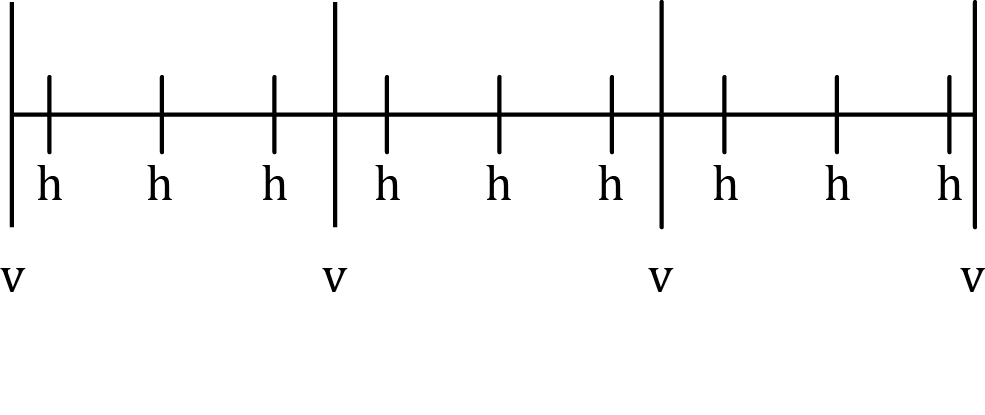
\includegraphics[keepaspectratio, width=4in]{1d_mapping_2.png}
  \end{center}
  \vspace{-.2in} % corrects bad spacing
  \caption{\label{fig:1d-projection} Projecting onto the parametric representation.}
\end{figure}

\begin{lemma}\label{lemma:h-extension}
	A sequence $\alpha$ is a valid collision sequence iff there exists at least one valid collision sequence containing $\alpha$ that starts and ends with an h.
\end{lemma}

Because of Lemma \ref{lemma:h-extension}, we will confine ourselves to only looking at collision sequences that start and end with an h.

\begin{definition}
	Given a collision sequence $\alpha$, define a sequence $\beta$ where each element $\beta_i$ is the number of v collisions between the i\textsuperscript{th} and (i+1)\textsuperscript{th} h in $\alpha$.
\end{definition}

The $\beta$ sequence is much simpler to think of geometrically in terms of our parametric representation shown in Figure \ref{fig:1d-projection}. $\beta_i$ represents the number of v collision tick marks in between each h collision tick mark.

\begin{figure}[H]
  \begin{center}
    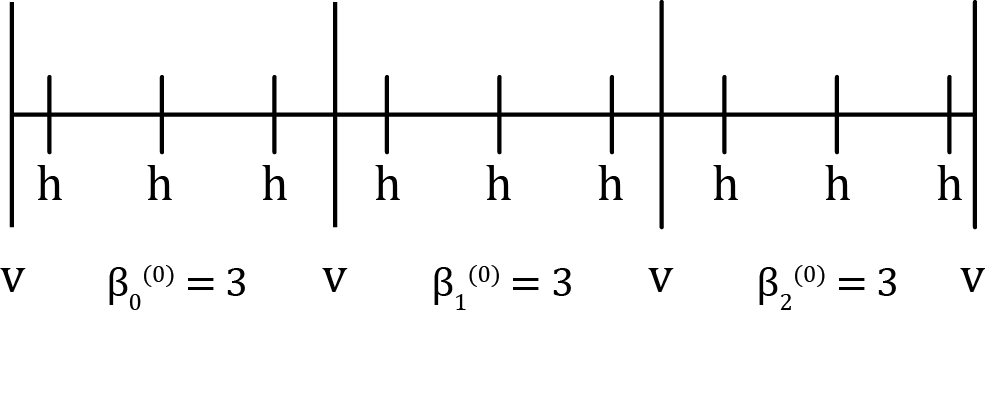
\includegraphics[keepaspectratio, width=4in]{1d_mapping_3.png}
  \end{center}
  \vspace{-.2in} % corrects bad spacing
  \caption{\label{fig:beta-sequence} The $\beta$ sequence.}
\end{figure}

\begin{lemma}\label{lemma:beta_pos}
	For every valid collision sequence, the following must be true

	\begin{equation}
		\beta_{min} > 0
	\end{equation}
\end{lemma}

\begin{proof}
	TODO
\end{proof}

\begin{theorem}\label{thm:beta_exremum}
	For every valid collision sequence, the following must be true
	
	\begin{equation}
		\beta_{max} - \beta_{min} \le 1
	\end{equation}
\end{theorem}

\begin{proof}

From Equation \ref{eq:parametric-line}, v collisions occur every $\Delta t = 1$ and h collisions occur every $\Delta t = m$. Thus, the following must be true

\begin{equation}
	\beta_i \in \paren{\floor{m}, \ceil{m}}
\end{equation}

For an $m$ to exist that satisfies the above constraints, all numbers in the $\beta$ sequence can only differ by 1.

\end{proof}

From now on we will only consider collision sequences, where $\beta$ starts and ends with $\beta_min$.

\begin{theorem}\label{thm:beta_i}
	Define 
	\begin{align}\label{delta_beta}
			\delta^{(\beta)}_i \coloneqq \begin{cases}
				x_0 \qquad &\text{if} \quad i = 0\\
				i (\beta_{max} - m) \qquad &\text{otherwise}
			\end{cases}
	\end{align}

	Then the following is true for all valid collision sequences

	\begin{align}\label{eq:beta_i}
		\beta_i = \floor{\delta^{(\beta)}_i} + \beta_{max} - \floor{\delta^{(\beta)}_{i+1}}
	\end{align}
\end{theorem}

\begin{proof}
	TODO...
\end{proof}

We can immediately notice that the $\delta^{(\beta)}$ sequence has the following features:

\begin{enumerate}
	\item The $\delta^{(\beta)}$ sequence is increasing, because $\beta_{max} \ge m$
	\item Combining Theorem \ref{thm:beta_exremum} and Equation \ref{eq:beta_i}, we get the following:

		\begin{align}
			\floor{\delta^{(\beta)}_{i+1}} - \floor{\delta^{(\beta)}_{i+1}}& = \beta_{max} - \beta_{min}\\
			& \le 1
		\end{align}
\end{enumerate}

Thus, if we plot the values of the $\delta^{(\beta)}$ sequence on a line, we notice something interesting: the plot looks very similar to our original plot of the collision sequence parameterized by $t$.

\begin{definition}
	Define a the sequence $C^{(0)}$ where each element $C^{(0)}_i$ is 1 more than the number of occurrences of $\beta_{max}$ between the i\textsuperscript{th} and (i+1)\textsuperscript{th} occurrence of $\beta_{min}$ in the $\beta$ sequence.
\end{definition} 

\begin{theorem}
	Define 
	\begin{align}\label{delta_c}
			\delta^{(C^{(j)})}_i \coloneqq \begin{cases}
				x_0 \qquad &\text{if} \quad i = 0\\
				i (C^{(j)}_{max} - m) \qquad &\text{otherwise}
			\end{cases}
	\end{align}

	Then the following is true for all valid collision sequences

	\begin{align}\label{eq:c_i}
		C^{(j)}_i = \floor{\delta^{(C^{(j)})}_i} + C^{(j)}_{max} - \floor{\delta^{(C^{(j)})}_{i+1}}
	\end{align}
\end{theorem} 

\begin{theorem}
	Define the sequence $a$ as

	\begin{align}
		a_0& \coloneqq 1\\
		a_1& \coloneqq \beta_{max} - m\\
		a_i& \coloneqq C^{(i-2)} a_{i-1} - a_{i-2} \qquad \text{for} \quad i \ge 2
	\end{align}

	For every valid collision sequence, $a \to 0$
\end{theorem}

\begin{proof}

\end{proof}